El objetivo de este capítulo será realizar una descripción y especificación de todas las características que componen este trabajo desde un punto de vista de la gestión del mismo. Desde la especificación de los requisitos, metodología de desarrollo, planificación y presupuesto. 

\section {Especificación de requisitos}

En el proceso de desarrollo de software, la especificación de requisitos es una etapa fundamental que establece las bases para el diseño y construcción de un sistema o aplicación \cite{mora2007especificacion}. Esta fase tiene como objetivo principal definir de manera clara y concisa tanto los requisitos.

Por un lado, se tienen los funcionales, que describen las funcionalidades específicas que el software debe ofrecer, y por otro lado los no funcionales, que se refieren a aspectos de rendimiento, seguridad, usabilidad y compatibilidadmora2007especificacion \cite{mora2007especificacion}.

A continuación se va a definir el formato en el que se presentarán estos requisitos. Este formato ha sido elegido al ser el más popular y utilizado durante nuestra formación, así como su alta capacidad de síntesis de la información y fácil comprensión. La tabla en cuestión tiene los siguientes campos:

\begin{itemize}
    \item Identificador: Sirve como identificador exclusivo de cada requisito, su formato se compone de los siguiente; RX-N, pudiendo tomar X los valores F (Funcional) o NF (No Funcional) y N como número del requisito dentro de su categoría (F o NF).
    \item Título: Describe de manera concisa el requisito.
    \item Prioridad: Define su nivel de importancia para el proyecto.
    \item Descripción: Describe el requisito de una manera más detallada.
\end{itemize}


\begin{table}[H] 
\begin{center}
\begin{tabular} {|P{4cm}|P{10cm}|}\hline
  \rowcolor{tables} {\bf Identificador} &{\bf RX - N}\\ \hline
  \cellcolor{tables}\textbf{Título}& \\ \hline
  \cellcolor{tables}\textbf{Prioridad}& Alta / Media / Baja  \\ \hline
  \cellcolor{tables}\textbf{Descripción}& \\ \hline
\end{tabular}
\end{center}
\vspace{-0.6cm}
\caption{Plantilla de requisitos}
\end{table}


\subsection {Requisitos Funcionales}
\begin{table}[H] 
\begin{center}
\begin{tabular} {|P{4cm}|P{10cm}|}\hline
  \rowcolor{tables} {\bf Identificador} &{\bf RF - 01}\\ \hline
  \cellcolor{tables}\textbf{Título}& Lectura del dataset\\ \hline
  \cellcolor{tables}\textbf{Prioridad}& Alta \\ \hline
  \cellcolor{tables}\textbf{Descripción}&
  El sistema deberá ser capaz de cargar y leer el dataset para su posterior uso y modificación durante el proyecto. \\ \hline
\end{tabular}
\end{center}
\vspace{-0.6cm}
\caption{Requisito Funcional 01}
\end{table}

\subsection {Requisitos Funcionales}
\begin{table}[H] 
\begin{center}
\begin{tabular} {|P{4cm}|P{10cm}|}\hline
  \rowcolor{tables} {\bf Identificador} &{\bf RF - 02}\\ \hline
  \cellcolor{tables}\textbf{Título}& Análisis de la distribución de clases\\ \hline
  \cellcolor{tables}\textbf{Prioridad}& Alta \\ \hline
  \cellcolor{tables}\textbf{Descripción}& 
  El sistema deberá analizar la distribución de las clases en el dataset para conocer las de mayor frecuencia, siendo las clases 'YES', 'NO' para la clasificación binaria, y 'Direct', 'Reported' y 'Judgmental' para la multi clase como se muestra en la introducción\\ \hline
\end{tabular}
\end{center}
\vspace{-0.6cm}
\caption{Requisito Funcional 02}
\end{table}

\subsection {Requisitos Funcionales}
\begin{table}[H] 
\begin{center}
\begin{tabular} {|P{4cm}|P{10cm}|}\hline
  \rowcolor{tables} {\bf Identificador} &{\bf RF - 03}\\ \hline
  \cellcolor{tables}\textbf{Título}& Procesamiento de la entrada de la tarea 1\\ \hline
  \cellcolor{tables}\textbf{Prioridad}& Alta  \\ \hline
  \cellcolor{tables}\textbf{Descripción}&  Supongamos que las seis anotaciones de un tweet fueron NO ,YES ,NO, YES ,YES ,YES , entonces el valor asignado al tweet será YES. Sin embargo, el número de etiquetas positivas (1 para indicar que el tweet es sexista) y el número de etiquetas negativas (0 para indicar que el tweet no tiene un contenido sexista), entonces se le asignará el valor X, porque es la clase más frecuente en el dataset\\ \hline
\end{tabular}
\end{center}
\vspace{-0.6cm}
\caption{Requisito Funcional 03}
\end{table}


\subsection {Requisitos Funcionales}
\begin{table}[H] 
\begin{center}
\begin{tabular} {|P{4cm}|P{10cm}|}\hline
  \rowcolor{tables} {\bf Identificador} &{\bf RF - 04}\\ \hline
  \cellcolor{tables}\textbf{Título}& Procesamiento de la entrada de la tarea 2\\ \hline
  \cellcolor{tables}\textbf{Prioridad}& Alta  \\ \hline
  \cellcolor{tables}\textbf{Descripción}&  La misma idea que aplicada a la tarea 1 solo que en lugar de elegir entre dos clases se elije entre 3\\ \hline
\end{tabular}
\end{center}
\vspace{-0.6cm}
\caption{Requisito Funcional 04}
\end{table}


\begin{table}[H] 
\begin{center}
\begin{tabular} {|P{4cm}|P{10cm}|}\hline
  \rowcolor{tables} {\bf Identificador} &{\bf RF- 05}\\ \hline
  \cellcolor{tables}\textbf{Título}& Preprocesado de los textos (tweets)\\ \hline
  \cellcolor{tables}\textbf{Prioridad}& Media \\ \hline
  \cellcolor{tables}\textbf{Descripción}& Antes de pasar los textos a nuestros modelos, es necesario procesarlos y transformarlos en vectores. En el preprocesamiento, también se eliminarán ciertas palabras del texto original como las palabras vacías (stop-words), signos de puntuación, números y otros tokens que pueden generar ruido en el entrenamiento del modelo, y que no ayudan en la tarea de clasificación porque no tienen contenido semántico. \\ \hline
\end{tabular}
\end{center}
\vspace{-0.6cm}
\caption{Requisito Funcional 05}
\end{table}

\begin{table}[H] 
\begin{center}
\begin{tabular} {|P{4cm}|P{10cm}|}\hline
  \rowcolor{tables} {\bf Identificador} &{\bf RF- 06}\\ \hline
  \cellcolor{tables}\textbf{Título}& Segmentación estratificada del dataset\\ \hline
  \cellcolor{tables}\textbf{Prioridad}& Alta  \\ \hline
  \cellcolor{tables}\textbf{Descripción}& Para poder entrenar y evaluar nuestros modelos, es necesario crear tres particiones del dataset original para obtener las particiones de training (80\% de los textos), validation (10\%) y test (10\%). Mientras que los dos primeros conjuntos se utilizan para entrenar y ajustar cada modelo, el último se utiliza para proporcionar una evaluación final del modelo. Esta división se realizará de forma aleatoria, pero garantizando que la distribución de clases en cada partición es similar a la del dataset original. \\ \hline
\end{tabular}
\end{center}
\vspace{-0.6cm}
\caption{Requisito Funcional 06}
\end{table}

\begin{table}[H] 
\begin{center}
\begin{tabular} {|P{4cm}|P{10cm}|}\hline
  \rowcolor{tables} {\bf Identificador} &{\bf RF- 07}\\ \hline
  \cellcolor{tables}\textbf{Título}& Tokenización de las entradas\\ \hline
  \cellcolor{tables}\textbf{Prioridad}& Alta  \\ \hline
  \cellcolor{tables}\textbf{Descripción}& Para que el sistema pueda usar los textos es imperativo llevar a cabo una tokenización adecuada de los mismos pasando de valores de texto a tokens, y estos a vectores con un valor asociado dentro de un espacio vectorial, que serán la entrada de nuestros modelos como se cuenta con detalle en la \autoref{tokenización}.\\ \hline
\end{tabular}
\end{center}
\vspace{-0.6cm}
\caption{Requisito Funcional 07}
\end{table}

\begin{table}[H] 
\begin{center}
\begin{tabular} {|P{4cm}|P{10cm}|}\hline
  \rowcolor{tables} {\bf Identificador} &{\bf RF- 08}\\ \hline
  \cellcolor{tables}\textbf{Título}& Entrenamiento y validación de modelos\\ \hline
  \cellcolor{tables}\textbf{Prioridad}& Media\\ \hline
  \cellcolor{tables}\textbf{Descripción}&  El sistema deberá ser capaz de para cada modelo entrenar con el dataset de entrenamiento proporcionado y realizar una posterior validación de los modelos con el dataset de validación\\ \hline
\end{tabular}
\end{center}
\vspace{-0.6cm}
\caption{Requisito Funcional 08}
\end{table}

\begin{table}[H] 
\begin{center}
\begin{tabular} {|P{4cm}|P{10cm}|}\hline
  \rowcolor{tables} {\bf Identificador} &{\bf RF- 09}\\ \hline
  \cellcolor{tables}\textbf{Título}& Clasificación de textos sexistas y no sexistas\\ \hline
  \cellcolor{tables}\textbf{Prioridad}& Alta  \\ \hline
  \cellcolor{tables}\textbf{Descripción}& En la tarea 1, el sistema (es decir, cada uno de los modelos propuestos) deberá inferir para cada texto, si su contenido es sexista.\\ \hline
\end{tabular}
\end{center}
\vspace{-0.6cm}
\caption{Requisito Funcional 09}
\end{table}

\begin{table}[H] 
\begin{center}
\begin{tabular} {|P{4cm}|P{10cm}|}\hline
  \rowcolor{tables} {\bf Identificador} &{\bf RF- 10}\\ \hline
  \cellcolor{tables}\textbf{Título}& Clasificación en la tarea 2\\ \hline
  \cellcolor{tables}\textbf{Prioridad}& Alta  \\ \hline
  \cellcolor{tables}\textbf{Descripción}& En la tarea 2,  el sistema (es decir, cada uno de los modelos propuestos) deberá inferir para cada texto, a qué clase pertenece: direct, Judgmental y reported. Estas clases fueron descritas en detalle en el \autoref{introducción}\\ \hline
\end{tabular}
\end{center}
\vspace{-0.6cm}
\caption{Requisito Funcional 10}
\end{table}

\begin{table}[H] 
\begin{center}
\begin{tabular} {|P{4cm}|P{10cm}|}\hline
  \rowcolor{tables} {\bf Identificador} &{\bf RF- 11}\\ \hline
  \cellcolor{tables}\textbf{Título}& Evaluación\\ \hline
  \cellcolor{tables}\textbf{Prioridad}& Alta  \\ \hline
  \cellcolor{tables}\textbf{Descripción}& Una vez entrenados los modelos, cada uno de ellos debe ser evaluado con las siguientes métricas sobre el conjunto test: Accuracy, Precisión, , Recall, F1 y sus versiones macros.\\ \hline
\end{tabular}
\end{center}
\vspace{-0.6cm}
\caption{Requisito Funcional 11}
\end{table}

\begin{table}[H] 
\begin{center}
\begin{tabular} {|P{4cm}|P{10cm}|}\hline
  \rowcolor{tables} {\bf Identificador} &{\bf RF- 12}\\ \hline
  \cellcolor{tables}\textbf{Título}& Matrices de confusión\\ \hline
  \cellcolor{tables}\textbf{Prioridad}& Alta  \\ \hline
  \cellcolor{tables}\textbf{Descripción}& Además de proporcionar los resultados de cada modelo sobre el conjunto test, el sistema también debe generar la matriz de confusión para cada uno de ellos.\\ \hline
\end{tabular}
\end{center}
\vspace{-0.6cm}
\caption{Requisito Funcional 12}
\end{table}

\subsection {Requisitos No Funcionales}

\begin{table}[H] 
\begin{center}
\begin{tabular} {|P{4cm}|P{10cm}|}\hline
  \rowcolor{tables} {\bf Identificador} &{\bf RNF- 01}\\ \hline
  \cellcolor{tables}\textbf{Título}& Uso de Google Collaboratory\\ \hline
  \cellcolor{tables}\textbf{Prioridad}& Alta \\ \hline
  \cellcolor{tables}\textbf{Descripción}& Se deberán poder usar las diferentes partes que componen al sistema en Google Collaboratory \\ \hline
\end{tabular}
\end{center}
\vspace{-0.6cm}
\caption{Requisito No Funcional 1}
\end{table}


\begin{table}[H] 
\begin{center}
\begin{tabular} {|P{4cm}|P{10cm}|}\hline
  \rowcolor{tables} {\bf Identificador} &{\bf RNF- 02}\\ \hline
  \cellcolor{tables}\textbf{Título}& Código Abierto\\ \hline
  \cellcolor{tables}\textbf{Prioridad}&  Media\\ \hline
  \cellcolor{tables}\textbf{Descripción}& El proyecto deberá ser de libre acceso garantizando el codigo abierto a través de la plataforma \href{https://github.com/ValenUC3M/-NLP-BachelorThesis-GonzaloValenti}{github}\\ \hline
\end{tabular}
\end{center}
\vspace{-0.6cm}
\caption{Requisito No Funcional 2}
\end{table}

\begin{table}[H] 
\begin{center}
\begin{tabular} {|P{4cm}|P{10cm}|}\hline
  \rowcolor{tables} {\bf Identificador} &{\bf RNF- 03}\\ \hline
  \cellcolor{tables}\textbf{Título}& Capacidades de uso\\ \hline
  \cellcolor{tables}\textbf{Prioridad}&  Alta\\ \hline
  \cellcolor{tables}\textbf{Descripción}& El sistema no deberá superar las capacidades ofrecidad por la herramienta Google Collaboratory descrita en la \autoref{entorno}\\ \hline
\end{tabular}
\end{center}
\vspace{-0.6cm}
\caption{Requisito No Funcional 3}
\end{table}

\begin{table}[H] 
\begin{center}
\begin{tabular} {|P{4cm}|P{10cm}|}\hline
  \rowcolor{tables} {\bf Identificador} &{\bf RNF- 04}\\ \hline
  \cellcolor{tables}\textbf{Título}& Python\\ \hline
  \cellcolor{tables}\textbf{Prioridad}&  Alta\\ \hline
  \cellcolor{tables}\textbf{Descripción}& El lenguaje de desarrollo debe ser Python\\ \hline
\end{tabular}
\end{center}
\vspace{-0.6cm}
\caption{Requisito No Funcional 4}
\end{table}


\section{Metodología de desarrollo}

Como ya se ha comentado anteriormente para este trabajo se ha optado por realizar el proceso estándar a la hora de desarrollar un proyecto de software. Como se ha estudiado en el Grado de Ingeniería Informática, la metodología iterativa e incremental conocida como Agile \cite{luna2019usabilidad} es una de las más adecuadas para este proyecto ya que es una metodología que trae consigo múltiples beneficios. Se destaca por su capacidad de adaptarse a los cambios y entregar incrementos de trabajo funcionales de forma continua. Fomenta la colaboración y la comunicación efectivas, así como un enfoque en la calidad y la mejora continua. Además, promueve la transparencia y la visibilidad en todas las etapas del proyecto. En resumen, Agile ofrece flexibilidad, entregas rápidas, colaboración, calidad, mejora constante y transparencia \cite{luna2019usabilidad} que se consideran fundamentales para el correcto desarrollo del proyecto.

De nuevo basándonos en lo aprendido la metodología de desarrollo será iterativa \cite{gutierrez2011metodos}, de tal manera que se siga un orden iterativo de desarrollo pudiendo regresar a anteriores fases del desarrollo para corregir y adaptar el proyecto conforme avance.

El proyecto se ha compuesto de las siguientes fases estándar para un proyecto de desarrollo de software:

\begin{itemize}
    \item Estudio del estado del arte: Estudiar de manera detallada las diferentes tareas asociadas con el proyecto para comprender bien el proceso y obtener posibles ideas y aplicaciones.
    \item Análisis del sistema: Analizar las diferentes características que debe tener el sistema para que funcione correctamente realizando una especificación de los requisitos tanto funcionales como no funcionales.
    \item Desarrollo del sistema: Crear, probar y adaptar un sistema informático capaz de realizar todas las tareas necesarias para realizar el proyecto.
    \item Evaluación del sistema: Una vez generado el sistema se deberá realizar una evaluación de los resultados obtenidos para los diferentes modelos con el objetivo de realizar a posteriori un análisis general de todos los resultados obtenidos.
    \item Desarrollo de la documentación: Para el correcto entendimiento del proyecto y con el objetivo de guardar un registro claro de todo lo requerido para realizar este proyecto se deberá realizar una documentación extensa y detallada que cubra todos los apartados del proyecto ya que la documentación en un proyecto de desarrollo de software es crucial al facilitar la comunicación efectiva entre las partes interesadas, registra las decisiones tomadas, permite el mantenimiento y la escalabilidad del software, facilita la transferencia de conocimiento y asegura el cumplimiento de regulaciones.
\end{itemize}

\section{Planificación del proyecto}

El proyecto se inició el 11 de enero de 2023 y finaliza el 17 de Junio de 2023. En total se han empleado 580 horas para las diferentes fases que han compuesto al proyecto como se muestra a continuación:

\begin{table}[H]
\begin{tabular}{|
>{\columncolor[HTML]{9B9B9B}}c |
>{\columncolor[HTML]{C0C0C0}}c |
>{\columncolor[HTML]{C0C0C0}}c |
>{\columncolor[HTML]{C0C0C0}}c |}
\hline
{\color[HTML]{000000} \textbf{Fases}}           
& \cellcolor[HTML]{9B9B9B}{\color[HTML]{000000} \textbf{Horas}} 
& \cellcolor[HTML]{9B9B9B}{\color[HTML]{000000} \textbf{Fecha de Inicio}}
& \cellcolor[HTML]{9B9B9B}{\color[HTML]{000000} \textbf{Fecha de Fin}} \\ \hline
{\color[HTML]{000000} \textbf{Estado del arte}} 
& {\color[HTML]{000000} 43}                                    
& {\color[HTML]{000000} 11/01/23}                                      
& {\color[HTML]{000000} 27/01/23}                                      
\\ \hline
\textbf{Análisis del sistema}                  
& 96                                                            
& 23/01/23                                                        
& 28/02/23                                                             
\\ \hline
\textbf{Desarrollo del sistema}                
& 207                                                         
& 20/02/23                                                        
& 17/04/23                                                       
\\ \hline
\textbf{Evaluación del sistema}              
& 110                                                       
& 15/04/23                                                        
& 10/05/23                                                       
\\ \hline
\textbf{Documentación}                     
& 167                                                         
& 28/04/23                                                     
& 16/06/23                                                 
\\ \hline
\textbf{Total}                                
& 580                                                          
& 11/01/23                                                        
& 16/06/23                                                         
\\ \hline
\end{tabular}
\caption{Tabla con el tiempo empleado para cada una de las fases del proyecto}
\end{table}

A continuación se muestra el diagrama de GANT para ofrecer una perspectiva visual de la planificación del proyecto:

\begin{figure}[H]
    \centering
    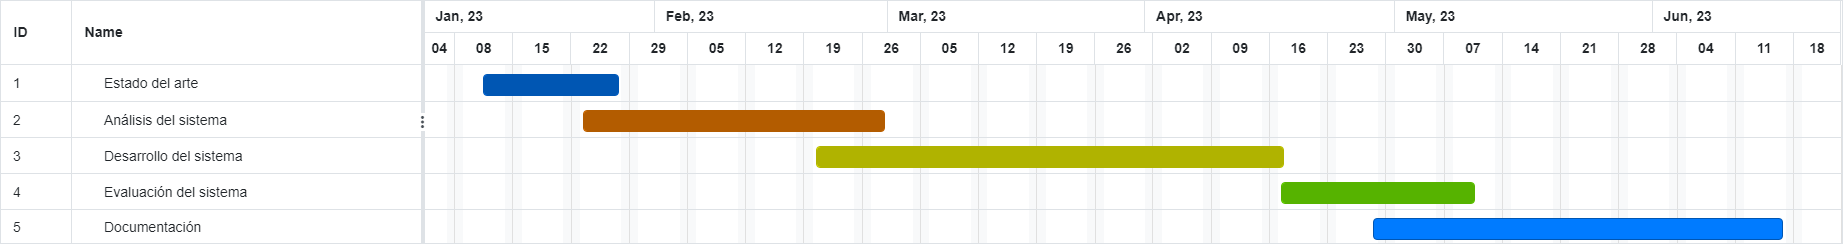
\includegraphics[width=16cm]{imagenes/Gestion/gant.png}
    \caption{\centering diagrama de gant del proyecto}
\end{figure}


\section{Presupuesto y Costes}

En esta sección se presenta el presupuesto del proyecto. Al tratarse de un proyecto individual bajo la supervisión de la tutora Isabel Segura Bedmar, se le asigna el puesto de Técnico de desarrollo a Gonzalo Valenti Sanguino cuya labor es la elaboración del proyecto siguiendo las directivas proporcionadas por su tutora. Dado que el periodo de elaboración del trabajo es del 11 de enero de 2023 al 16 de Julio de 2023 se distribuirán los salarios de manera acorde a esos 5 meses basándonos las \href{https://www.uc3m.es/pdi/media/pdi/doc/archivo/doc_tablas-retributivas-mayo22/tablas-retributivas_contratos-proyectos_30052022.pdf}{tablas retributivas} definidas por el Vicerrectorado el 30 de Mayo de 2022.

Por un lado el sueldo establecido a Isabel Segura es el de Doctor A+ (2.023,81 Euros mensuales) y a Gonzalo Valenti es Especialista C (1.383.33€)


A continuación se muestran la tabla tanto de presupuestos como costes finales asociados al personal del proyecto:

\begin{table}[H]
\begin{tabular}{|c|c|c|c|c|c|}
\hline
\rowcolor[HTML]{9B9B9B} 
\cellcolor[HTML]{9B9B9B}{\color[HTML]{000000} \textbf{Personal}} 
& \cellcolor[HTML]{9B9B9B}{\color[HTML]{000000} \textbf{Sueldo/Hora}} 
& \textbf{Horas/Mes}
& \textbf{Sueldo/Mes}         
& \textbf{Meses} 
& \textbf{Sueldo total}     
\\ \hline
\rowcolor[HTML]{C0C0C0} 
{\color[HTML]{000000} \textbf{Isabel Segura}}                  
& \cellcolor[HTML]{C0C0C0}{\color[HTML]{000000} 11.5€}             
& 30                
& \cellcolor[HTML]{C0C0C0}345€ & 2            
& \cellcolor[HTML]{C0C0C0}690€ \\ \hline
\rowcolor[HTML]{C0C0C0} 
{\color[HTML]{000000} \textbf{Gonzalo Valenti}}              
& {\color[HTML]{000000} 7.86€}                                  
& 116                
& 911,76€                     
& 5             
& 4.558,8€                   
\\ \hline
\end{tabular}
\caption{Tabla de costes asociados al personal del proyecto}
\end{table}

A su vez hay que tener en cuenta los costes asociados las diferentes herramientas de software y hardware usadas durante el proyecto. La herramienta principal es un ordenador de sobremesa custom montado a piezas junto a dos monitores, teclado, ratón y silla, además de una licencia de Windows 10:

\begin{table}[H]
\begin{tabular}{|c|c|}
\hline
\rowcolor[HTML]{9B9B9B} 
{\color[HTML]{000000} \textbf{Descripción}}                   
& {\color[HTML]{000000} \textbf{Coste}}                
\\ \hline
\rowcolor[HTML]{C0C0C0} 
{\color[HTML]{000000} Ordenador sobremesa}                 
& {\color[HTML]{000000} 1079€}                          
\\ \hline
\rowcolor[HTML]{C0C0C0} 
{\color[HTML]{000000} Periféricos}                           
& {\color[HTML]{000000} 212,57€}                     
\\ \hline
\rowcolor[HTML]{C0C0C0} 
\multicolumn{1}{|l|}{\cellcolor[HTML]{C0C0C0} Windows 10 Home} 
& \multicolumn{1}{l|}{\cellcolor[HTML]{C0C0C0} 145€}      
\\ \hline
\rowcolor[HTML]{C0C0C0} 
\multicolumn{1}{|l|}{\cellcolor[HTML]{C0C0C0} Total}         
& \multicolumn{1}{l|}{\cellcolor[HTML]{C0C0C0} 1.436,57€} 
\\ \hline
\end{tabular}
\caption{Coste asociado a las herramientas de hardware y software del proyecto}
\end{table}

Cabe destacar que al ser un ordenador por piezas se ha marcado como referencia para su valor un ordenador equivalente en componentes como el que se muestra en la siguiente referencia \cite{pcomp}.


Adicionalmente se ha usado material de oficina, así como electricidad e internet para poder usar adecuadamente el equipo informático por lo que a continuación se muestra los costes asociados a los mismos:

\begin{table}[H]
\begin{tabular}{|c|c|}
\hline
\rowcolor[HTML]{9B9B9B} 
{\color[HTML]{000000} \textbf{Descripción}}                   
& {\color[HTML]{000000} \textbf{Coste}}                
\\ \hline
\rowcolor[HTML]{C0C0C0} 
{\color[HTML]{000000} Material de oficina}                 
& {\color[HTML]{000000} 45€}                          
\\ \hline
\rowcolor[HTML]{C0C0C0} 
{\color[HTML]{000000} Electricidad}                           
& {\color[HTML]{000000} 385€}                     
\\ \hline
\rowcolor[HTML]{C0C0C0} 
\multicolumn{1}{|l|}{\cellcolor[HTML]{C0C0C0} Internet} 
& \multicolumn{1}{l|}{\cellcolor[HTML]{C0C0C0} 57,90€}      
\\ \hline
\rowcolor[HTML]{C0C0C0} 
\multicolumn{1}{|l|}{\cellcolor[HTML]{C0C0C0} Total}         
& \multicolumn{1}{l|}{\cellcolor[HTML]{C0C0C0} 487,90€} 
\\ \hline
\end{tabular}
\caption{Coste indirectos}
\end{table}

Al tratarse de proyecto de investigación sin ánimo de lucro los beneficios son nulos por lo que el desglose de costes finales queda de la siguiente manera:

\begin{table}[H]
\begin{tabular}{|c|c|}
\hline
\rowcolor[HTML]{9B9B9B} 
{\color[HTML]{000000} \textbf{Descripción}}                   
& {\color[HTML]{000000} \textbf{Coste}}                
\\ \hline
\rowcolor[HTML]{C0C0C0} 
{\color[HTML]{000000} Personal}                 
& {\color[HTML]{000000} 5.248,8€}                          
\\ \hline
\rowcolor[HTML]{C0C0C0} 
{\color[HTML]{000000} Hardware y Software}                           
& {\color[HTML]{000000} 1.436,57€}                     
\\ \hline
\rowcolor[HTML]{C0C0C0} 
\multicolumn{1}{|l|}{\cellcolor[HTML]{C0C0C0}Material} 
& \multicolumn{1}{l|}{\cellcolor[HTML]{C0C0C0}487,90€}      
\\ \hline
\rowcolor[HTML]{C0C0C0} 
\multicolumn{1}{|l|}{\cellcolor[HTML]{C0C0C0}Total}         
& \multicolumn{1}{l|}{\cellcolor[HTML]{C0C0C0}7.173,27€} 
\\ \hline
\end{tabular}
\caption{Coste asociado a las herramientas de hardware y software del proyecto}
\end{table}